\documentclass[pdftex,11pt]{article}
\usepackage[pdftex]{graphicx}
\usepackage{enumerate}
\usepackage{amsmath}
\usepackage{amssymb}
\usepackage{multicol}
\usepackage{algpseudocode}
\usepackage{algorithm}
\usepackage{algorithm}
\usepackage{geometry}
\usepackage{float}
\geometry{verbose,tmargin=1in,bmargin=1in,lmargin=1in,rmargin=1in}

\begin{document}
\title{COMP 540 Statistical Machine Learning}
\author{Xiang Zhou (xz58) - Guangyuan Yu ()}
\date{2017.01.17}
\maketitle
\newcommand{\pr}{\mathbb{P}}
\begin{enumerate}
\item The code is in sampler.py

For the UnivariateNormal sampler, I generated a random number from
the uniform distribution {[}0,1{]} , and use the inverse Gaussian
error functionn to get the answer.
\begin{enumerate}
\item For the MultivariateNormal sampler, I followed the steps on the linked
wikipedia page. By using the Cholesky decomposition, I find the suitable
matrix and generating independent normal values .
\item For the Categorical sampler, since an array of probabilities is given
during initialization, I simply generated a number {[}0,1{]} and found
the correct partial sum iterating through the array.
\item For the MixtureModel sampler, I used a Categorical sampler to pick
the right probability model to use, then sampled using that probability
model.
\end{enumerate}
\item Let $X_0 \sim Pois(\lambda_0)$ and $X_1 \sim Pois(\lambda_1)$. Thus:\\
\begin{center}
$P(X_0 = k_0) = \frac{\lambda_0^{k_0}e^{-\lambda_0}}{k_0!}$ and $P(X_1 = k_1) = \frac{\lambda_1^{k_1}e^{-\lambda_1}}{k_1!}$
\end{center}For some $Y=X_{0}+X_{1}$:
\begin{align*}
P(Y=y)= & P(X_{0}+X_{1}=y)\\
= & f_{Y}(y)\\
= & \sum\limits _{j=0}^{y}f_{x_{0}}(j)f_{x_{1}}(y-j)\\
= & \sum\limits _{j=0}^{y}\frac{\lambda_{0}^{j}e^{-\lambda_{0}}}{j!}\frac{\lambda_{1}^{y-j}e^{-\lambda_{1}}}{(y-j)!}\\
= & \sum\limits _{j=0}^{y}\frac{\lambda_{0}^{j}\lambda_{1}^{y-j}}{j!(y-j)!}e^{-(\lambda_{0}+\lambda_{1})}\\
= & e^{-(\lambda_{0}+\lambda_{1})}\sum\limits _{j=0}^{y}\frac{y!}{j!(y-j)!}\frac{\lambda_{0}^{j}\lambda_{1}^{y-j}}{y!}\\
= & e^{-(\lambda_{0}+\lambda_{1})}\sum\limits _{j=0}^{y}C_{y}^{j}\frac{\lambda_{0}^{j}\lambda_{1}^{y-j}}{y!}\\
= & e^{-(\lambda_{0}+\lambda_{1})}\frac{(\lambda_{0}+\lambda_{1})^{y}}{y!}
\end{align*}
\\
That is to say $Y\sim Pois(\lambda_{0}+\lambda_{1})$. QED.In the
last step, we use the characteristic of binomial expansion. 
\item Use the law of contingent probability
\begin{align*}
p(X_{1}=x_{1})= & \int_{-\infty}^{\infty}p(X_{1}=x_{1}|X_{0}=x_{0})p(X_{0}=x_{0})dx_{0}\\
\alpha_{1}e^{-\frac{(x_{1}-\mu_{1})^{2}}{2\sigma_{1}^{2}}}= & \int_{-\infty}^{\infty}\alpha e^{-\frac{(x_{1}-x_{0})^{2}}{2\sigma^{2}}}\alpha_{0}e^{-\frac{(x_{0}-\mu_{0})^{2}}{2\sigma_{0}^{2}}}dx_{0}\\
= & \alpha_{0}\alpha\int_{-\infty}^{\infty}e^{-(\frac{(x_{1}-x_{0})^{2}}{2\sigma^{2}}+\frac{(x_{0}-\mu_{0})^{2}}{2\sigma_{0}^{2}})}dx_{0}\\
= & \alpha_{0}\alpha\frac{\sigma\sigma_{0}\sqrt{2\pi}}{\sqrt{\sigma^{2}+\sigma_{0}^{2}}}e^{-\frac{(x_{1}-\mu_{0})^{2}}{2(\sigma_{0}^{2}+\sigma^{2})}}\\
\\
\end{align*}
In the last step, we use mathmatica to calculate the intergral. Therefore,
we find that:
\begin{align*}
\alpha_{1}= & \alpha_{0}\alpha\frac{\sigma\sigma_{0}\sqrt{2\pi}}{\sqrt{\sigma^{2}+\sigma_{0}^{2}}}\\
\mu_{1}= & \mu_{0}\\
\sigma_{1}= & \sqrt{\sigma_{0}^{2}+\sigma^{2}}
\end{align*}
according to normalization condition, we can get:
\[
\alpha=\frac{1}{\sqrt{2\pi}\sigma}
\]
\[
\alpha_{0}=\frac{1}{\sqrt{2\pi}\sigma_{0}}
\]
\[
\alpha_{1}=\frac{1}{\sqrt{2\pi}\sigma_{1}}
\]
\[
p(X_{1}=x_{1})=\alpha_{0}\alpha\frac{\sigma^{2}\sigma_{0}^{2}\sqrt{2\pi}}{\sqrt{\sigma^{2}+\sigma_{0}^{2}}}e^{-\frac{(x_{1}-\mu_{0})^{2}}{2(\sigma_{0}^{2}+\sigma^{2})}}=\frac{1}{\sqrt{2\pi}\sqrt{\sigma_{0}^{2}+\sigma^{2}}}e^{-\frac{(x_{1}-\mu_{0})^{2}}{2(\sigma_{0}^{2}+\sigma^{2})}}
\]
\item $A=\left(\begin{array}{cc}
13 & 5\\
2 & 4
\end{array}\right)$\\
We use tool box to find the eigenvalues are $\lambda=14$ and $\lambda=3$.\\
For $\lambda=14$:
\begin{align*}
\left(\begin{array}{cc}
13 & 5\\
2 & 4
\end{array}\right)\left(\begin{array}{c}
x\\
y
\end{array}\right)= & 14\left(\begin{array}{c}
x\\
y
\end{array}\right)\\
\left(\begin{array}{c}
-x+5y\\
2x-10y
\end{array}\right)= & \left(\begin{array}{c}
0\\
0
\end{array}\right)
\end{align*}
\\
We get $x=5y$ so the eigenvector is $\left(\begin{array}{c}
5\\
1
\end{array}\right)$.\\
For $\lambda=3$:
\begin{align*}
\left(\begin{array}{cc}
13 & 5\\
2 & 4
\end{array}\right)\left(\begin{array}{c}
x\\
y
\end{array}\right)= & 3\left(\begin{array}{c}
x\\
y
\end{array}\right)\\
\left(\begin{array}{c}
10x+5y\\
2x+y
\end{array}\right)= & \left(\begin{array}{c}
0\\
0
\end{array}\right)
\end{align*}
\\
We get $y=-2x$ so the eigenvector is $\left(\begin{array}{c}
1\\
-2
\end{array}\right)$.
\item Let A and B be $2\times2$ matrices

\begin{enumerate}
\item Let $A=\left(\begin{array}{cc}
1 & 2\\
3 & 4
\end{array}\right),B=\left(\begin{array}{cc}
5 & 6\\
7 & 8
\end{array}\right)$. 
\[
(A+B)^{2}=\left(\begin{array}{cc}
6 & 8\\
10 & 12
\end{array}\right)^{2}=\begin{array}{cc}
116 & 144\\
180 & 224
\end{array}
\]
\[
A^{2}+2A*B+B^{2}=\begin{array}{cc}
112 & 132\\
192 & 228
\end{array}
\]
\[
(A+B)^{2}\neq(A^{2}+2A*B+B^{2})
\]
\item If we have $A=\left(\begin{array}{cc}
2 & -1\\
2 & -1
\end{array}\right)$ and $B=\left(\begin{array}{cc}
1 & 4\\
2 & 8
\end{array}\right)$ .Then we can get $AB=\left(\begin{array}{cc}
0 & 0\\
0 & 0
\end{array}\right)$.
\end{enumerate}
\end{enumerate}

\section{Locally weighted linear regression}

	\subsection{}
	\begin{itemize}
		\item Since we have $\mu^T\mu = 1$, then:
		\begin{align*}
		A^TA 
		&= (I - 2\mu\mu^T)^T (I - 2\mu\mu^T) \\
		&= (I - 2\mu(\mu^T\mu)\mu^T)^T(I - 2\mu(\mu^T\mu)\mu^T)\\
		&= (I - 2(\mu\mu^T)^2)^T(I - 2(\mu\mu^T)^2)         &\Longrightarrow  uu^{T}=(uu^{T})^{2} \Longrightarrow  uu^{T}=I\\
		&= (I - 2I)^T(I - 2I)\\
		& =I\\
		\end{align*}
	\end{itemize}
	
	\subsection{}
	\begin{itemize}
		\item For given $f(x) = x^3$, we have $f^{\prime}(x)=3x^{2}$, $f^{\prime\prime}(x)=6x$, the second derivative is always greater than 0 when $x \geq 0$. Thus, we prove $f(x)$ is convex for $x \geq 0$.
		
		\item Assume $x = (x_{1}, x_{2}) \in \Re$, $y = (y_{1}, y_{2}) \in \Re$. Given the inequality provided in the assignment, we have to prove the following inequality:
		\begin{align*}
		f(\lambda(x_1, x_2) +(1-\lambda)(y_1, y_2)) \leq & \lambda f(x_1, x_2)+(1-\lambda)f(y_1, y_2)\\ 
		& \downarrow \\	
		f(\lambda x_1 + (1 - \lambda)y_1, \lambda x_2 + (1 - \lambda)y_2) \leq & \lambda f(x_1, x_2)+(1-\lambda)f(y_1, y_2)\\ 
		& \downarrow \\
		max\{\lambda x_1+(1-\lambda)y_1, \lambda x_2+(1-\lambda)y_2\} \leq & \lambda max\{x_1, x_2\} +(1-\lambda)max\{ y_1, y_2\} 
		\end{align*}
		Assume $x_1 > x_2$, $y_1 <= y_2$, then:
 		\begin{align*}
 			f(\lambda x_1 + (1 - \lambda)y_1, \lambda x_2 + (1 - \lambda)y_2)
 			& \leq \lambda x_1+ (1 - \lambda)y_2 \\
 			&= \lambda f(x_1, x_2) + (1 - \lambda)f(y_1, y_2)
 		\end{align*}
 		Assume $x_1 > x_2$, $y_1 > y_2$, then:
 		\begin{align*}
			f(\lambda x_1 + (1 - \lambda)y_1, \lambda x_2 + (1 - \lambda)y_2)
 			&= \lambda x_1 + (1 - \lambda)y_1 \\
 			&= \lambda f(x_1, y_1) + (1 - \lambda)f(x_2, y_2)
 		\end{align*} 
		For $x_1 <= x_2$, $y_1 > y_2$, and $x_1 <= x_2$, $y_1 <= y_2$, we can prove them similarly.\\
 		Hence, $f(x_1, x_2) = max(x_1, x_2)$ is a convex function in $\Re^2$.
		
		\item Assume function $h = f + g, (x, y \in S)$, according to the inequality, we have:
		\begin{align*}
			h(\lambda x + (1 - \lambda)y) 
			&=(f + g)(\lambda x + (1 - \lambda)y) \\
			&= f(\lambda x + (1 - \lambda)y) + g(\lambda x + (1 - \lambda)y)\\
 			&\leq \lambda f(x) + (1 - \lambda)f(y) + \lambda g(x) + (1 - \lambda)g(y) \\
 			&= \lambda h(x) + (1 - \lambda)h(y)
 		\end{align*}
		Thus, we have proved that $f+g$ is convex on $S$.
		
		\item To prove $fg$ is convex, we are going to prove the second derivative of $fg$ is greater than 0 on $S$
		\begin{align*}
			(fg)^{\prime\prime} 
			&= (fg^{\prime}+f^{\prime}g)^{\prime}\\
			&= fg^{\prime\prime}+2f^{\prime}g^{\prime}+f^{\prime\prime}g
		\end{align*} 
		Because univariate functions f and g are convex and non-negative on $S$, so $f^{\prime\prime}$ and $g^{\prime\prime}$ are greater than 0. Also, they have their minimum within $S$ at the same point, then $f^{\prime}g^{\prime} $ is greater than 0. Hence, we have proved that the second derivative of $fg$ is greater than 0 on $S$.
	\end{itemize}
	
	\subsection{}
	\begin{itemize}
		\item The constraint function for given $H(p)$ is:
		\begin{align*}
			g(p)=g(p_{1,}p_{2},...,p_{K})=\sum_{i=1}^{K}p_{i} = 1	
 		\end{align*}
		Then we have Lagrange function $L(p)$:
 		\begin{align*}
		L(p)=H(p)+\lambda(g(p)-c)\\
		\downarrow\\
 		L(p) = -\sum_{i = 1}^{K} p_i log(p_i) + \lambda (\sum_{i = 1}^{K} p_i - 1)
 		\end{align*}
 		Then calculate the derivative based on $p_i$:
 		\begin{align*}
		\frac{\partial L}{\partial p_{i}} &= -p_{i}\frac{1}{p_{i}}-log(p_{i})+\lambda\\
		&= - 1 - log(p_{i})+\lambda\\
		 &=0\\
		 \downarrow\\
		 p_i &= e^{\lambda - 1}
 		\end{align*}
		Since $\lambda$ is constant, we have all the $p_i$ of the same value:\\
		\begin{align*}
		\sum_{i=1}^{K}p_{i} &= 1\\
		 \downarrow\\
		p_{i} &= \frac{1}{K}
		\end{align*}
 		Therefore, we find that the categorical distribution has highest entropy when each category has the same probability.	
	\end{itemize}



\section{}
\begin{itemize}
\item Part 1 \begin{align*}
	J(\theta)&=\sum^m_{i=1}w^{(i)}(\theta^Tx^{(i)}-y^{(i)})^2\\&=(X\theta-y)^TW(X\theta-y)\\
	And : A&=X\theta-y\\&=
	\begin{pmatrix}
		x_1^{(1)} & \cdots & x_D^{(1)}\\
		\vdots & \ddots & \vdots\\
		x_1^{(N)} & \cdots & x_D^{(N)}
	\end{pmatrix}\\
	So that:
	J(\theta)&=A^TWA\\
	&=(x^{(1)^T}-y^{(1)}\cdots x^{(N)^T}\theta-y^{(N)})
	\begin{pmatrix}
		w^{(1)} & \cdots & 0\\
		\vdots & \ddots & \vdots\\
		0 & \cdots & w^{(n)}
	\end{pmatrix}
	\begin{pmatrix}
		x^{(1)^T}\theta-y^{(1)}\\
		\vdots\\
		x^{(N)^T}\theta-y^{(N)}
	\end{pmatrix}\\
	&=\sum^m_{i=1}w^{(i)}(x^{(i)^T}\theta-y^{(i)})^2\\
	&=w^{(i)}(\theta^Tx^{(i)}-y^{(i)})^2
	\end{align*}
\item Part 2 \begin{align*}
	J(\theta)&=(X\theta-y)^TW(X\theta-y)\\
	&=(\theta^TX^T-yT)W(X\theta-y)\\
	&=\theta^TX^TWX\theta-\theta^TX^TWXy-y^TWX\theta+y^TWy
	\end{align*}
	Because $(\theta^TX^TW)$ and $y$ are $1\times N$ and $N\times 1$ respectively, we have\\
	$$\theta^TX^TWy=y^TWX\theta$$
	And: $$\frac{dJ(\theta)}{d\theta}=\frac{d}{d\theta}[\theta^TX^TWX\theta]-2\frac{d}{d\theta}[\theta^TX^TWy]+\frac{d}{d\theta}[y^TWy]=0$$
	By taking the matrix derivative, we get:
	$$0=2X^TWX\theta-2X^TWy$$
	$$\hat{\theta}=(X^TWX)^{-1}X^TWy$$
\item Part 3

Calculating $\theta$ by Batch Gradient Descent:
 


Input data format: Data Matrix $X \in m\times d+1$, vector $y\in m\times 1$, learning rate $\alpha\in \mathbb{R}$, input vector $x\in\mathbb{R}^{d+1}$, bandwidth of sphere of influence around $x$ $\tau$\\
Output data format:Vector $\theta\in\mathbb{R}^{d+1}$ that minimizes weighted LSE\\

$$\theta\gets d\times 1 zeros matrix$$ 
$$w\gets m\times n zeros matrix$$ 
$$grad\gets d\times 1 zeros matrix$$ 
$$for (j=0 to m)$$
$$w_j^{(j)}\gets\frac{(x-X^{(j)})^T(x-X^{(j)})}{2\tau^2}$$
$$end for $$

$$For(j=0 to an arbitrary number)$$
$$grad\gets\frac{X^Tw(X\theta-y)}{m}$$
 $$\theta\gets\theta-\alpha*grad$$
 $$end for $$
 $$ Return\theta$$
\end{itemize}
\section{Properties of the linear regression estimator}
\begin{itemize}
\item Under the assumption that $E[\epsilon]=0$,
	\begin{align*}
		\theta&=(X^TX)^{-1}X^Ty\\
		E[\theta]&=E[(X^TX)^{-1}X^Ty]\\
		&=(X^TX)^{-1}X^TE[X\theta^*+\epsilon]\\
		&=(X^TX)^{-1}(X^TX)\theta^*+(X^TX)^{-1}X^TE[\epsilon]\\
		&=\theta^*+0=\theta^*
	\end{align*}
\item Under the assumption that $Var(\epsilon)=\sigma^2$,
	\begin{align*}
		Var(\theta)&=Var((X^TX)^{-1}X^Ty)\\
		&=Var((X^TX)^{-1}X^T(X\theta^*+\epsilon))\\
		&=Var(\theta^*)+Var((X^TX)^{-1}\epsilon)\\
		&=0+(X^TX)^{-1}Var(\epsilon)\\
		&=(X^TX)^{-1}\sigma^2
	\end{align*}
\end{itemize}

\section{Problem 3.1 Implementing linear regression}
\subsection{Implementing linear regression with one variable}

\begin{figure}[H]
  \caption{Plotting the data}
  \centering
    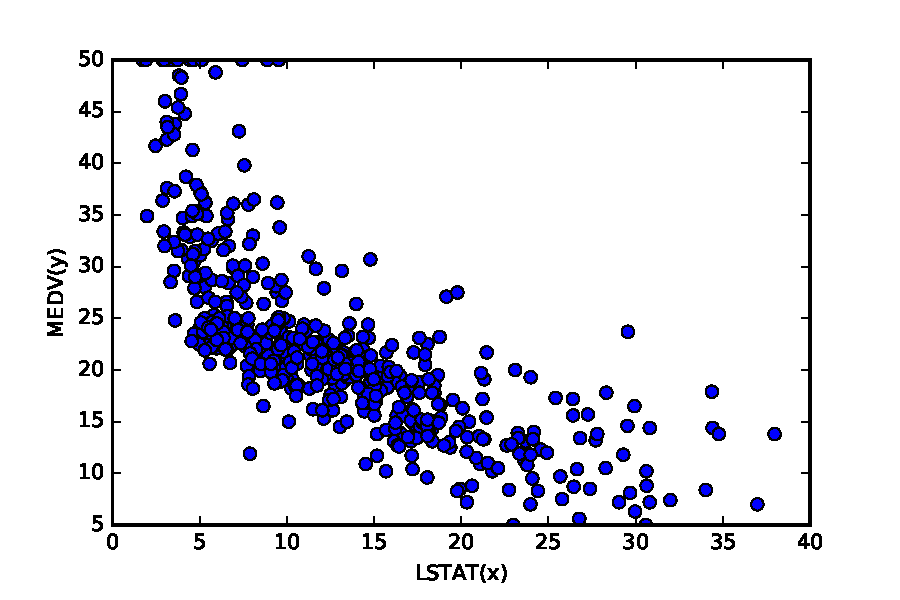
\includegraphics[scale=1]{fig1.pdf}
\end{figure}
\subsection{Problem 3.1 A1Computing the cost function J($\theta$)}
see our code 
\subsection{Problem 3.1 A2 Implmenting gradient descent}
\begin{figure}[H]
  \caption{Fitting a linear model to the data in fig 1}
  \centering
    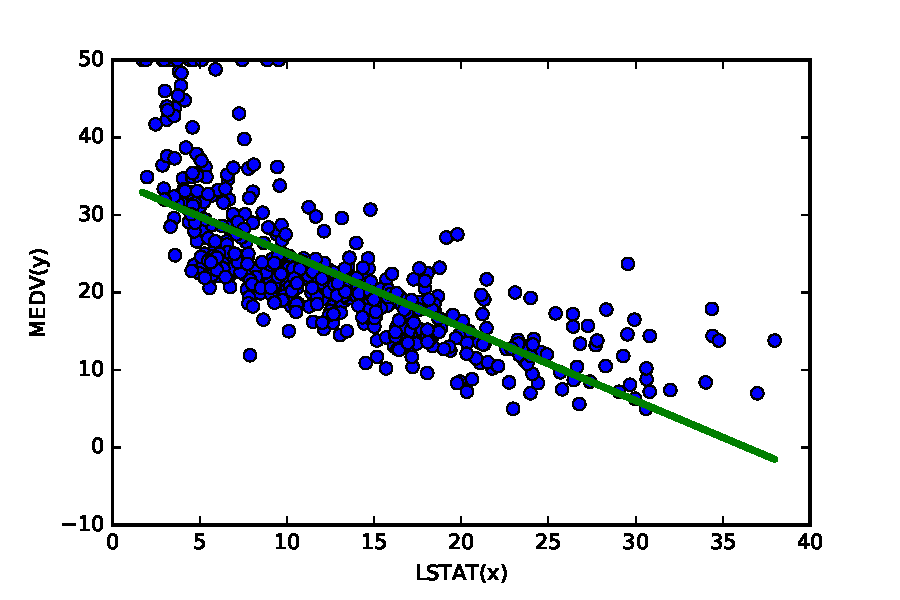
\includegraphics[scale=1]{fig2.pdf}
\end{figure}
\begin{figure}[H]
  \caption{convergence of gradient }
  \centering
    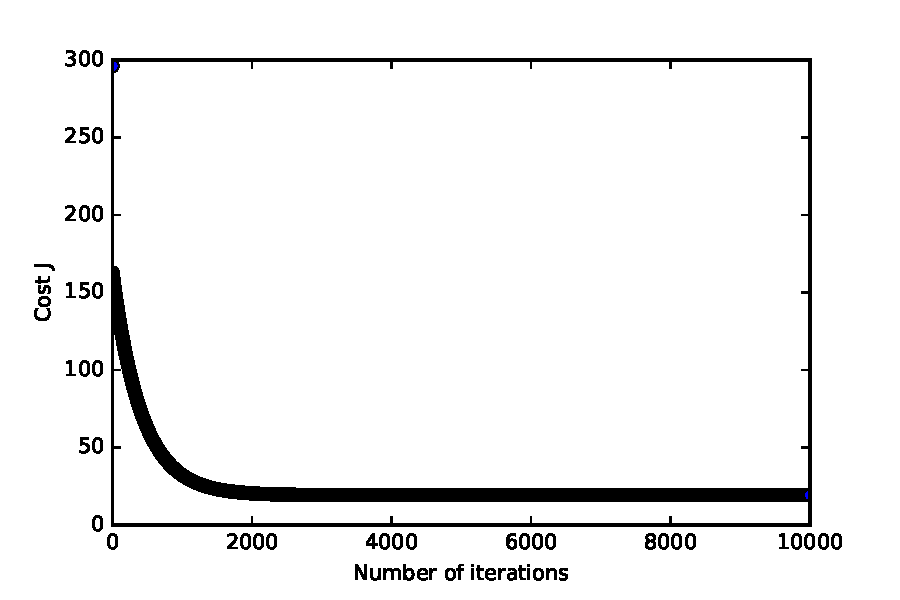
\includegraphics[scale=1]{fig4.pdf}
\end{figure}

\subsection{Problem 3.1 A3 Predicting on unseen data}
Theta found by gradient descent: [34.55363411  -0.95003694]
For lower status percentage = 5\%, we predict a median home value of 298034.494122
For lower status percentage = 50\%, we predict a median home value of -129482.128898
\begin{figure}[H]
  \caption{Surface plot of J}
  \centering
    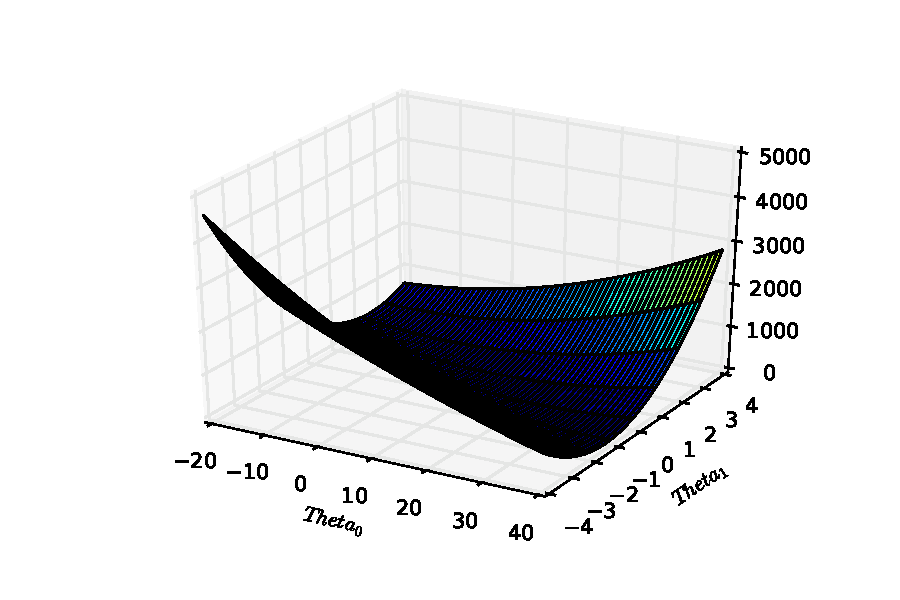
\includegraphics[scale=1]{fig3a.pdf}
\end{figure}
\begin{figure}[H]
  \caption{contour plot of J}
  \centering
    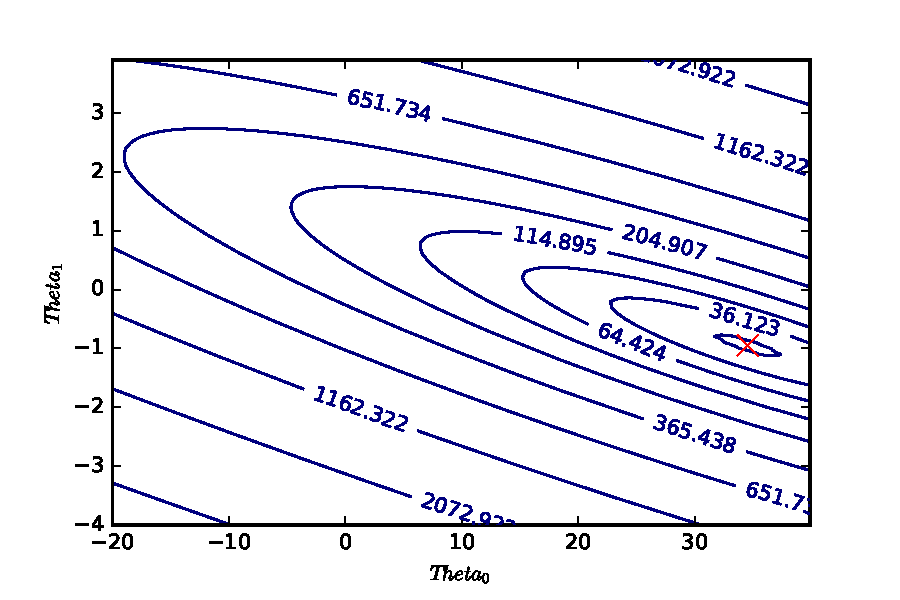
\includegraphics[scale=1]{fig3b.pdf}
\end{figure}
\subsection{assessing model quality}
The coefficients computed by sklearn:  34.5538408794  and  -0.950049353758
2  fold cross\_validation MSE =  39.5116296814
2  fold cross\_validation r\_squared =  0.510083569547

5  fold cross\_validation MSE =  42.61890333
5  fold cross\_validation r\_squared =  0.297106799977

10  fold cross\_validation MSE =  41.8292437273
10  fold cross\_validation r\_squared =  -0.18466981353
So k=2 is the best








\subsection{Problem 3.1 B Linear regression with multiple variables}
\subsection{Problem 3.1 B1Feature normalization}
see in the code
\subsection{Problem 3.1 B2 Loss function and gradient descent}
\begin{figure}[H]
  \caption{J for multiple variables}
  \centering
    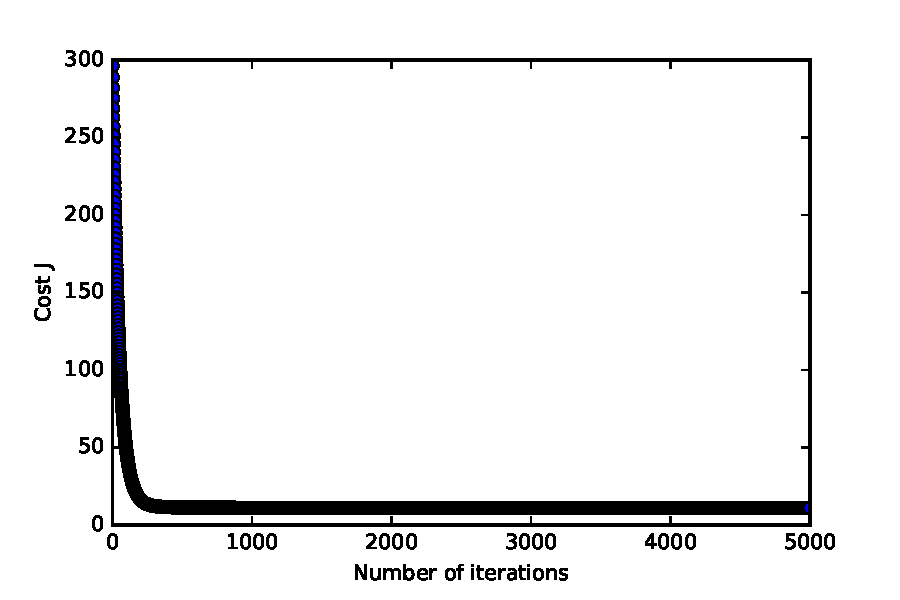
\includegraphics[scale=1]{fig5.pdf}
\end{figure}
Theta computed by gradient descent:  [  2.25328063e+01  -9.13925619e-01   1.06949712e+00   1.07531669e-01
   6.87258582e-01  -2.05340341e+00   2.67719690e+00   1.55788957e-02
  -3.10668099e+00   2.56946272e+00  -1.97453430e+00  -2.05873147e+00
   8.55982884e-01  -3.74517559e+00]

\subsection{Problem 3.1 B3 Making predictions on unseen data}

For average home in Boston suburbs, we predict a median home value of 225328.063241
The predictions match very well. Even though the theta are different but we can still have a good prediction because we have a lot of parameters. The difference of theta may come from the normalization of data.


\subsection{Problem 3.1 B4 Normal equation}

Theta computed by direct solution is:  [  3.64911033e+01  -1.07170557e-01   4.63952195e-02   2.08602395e-02
   2.68856140e+00  -1.77957587e+01   3.80475246e+00   7.51061703e-04
  -1.47575880e+00   3.05655038e-01  -1.23293463e-02  -9.53463555e-01
   9.39251272e-03  -5.25466633e-01]
For average home in Boston suburbs, we predict a median home value of 225328.063241


\subsection{Problem 3.1 B5 Convergence of gradient descent}
After running the four different learning rates provided (.01, .03, .1, and .3), we found that all converged, none with oscillation, on the same value. Thus, the best choice for a learning rate out of these four is 0.3 due to the fact that it converges the fastest and thus requires the least amount of iterations to finish training. 
\begin{figure}[H]
  \caption{J for different learning rate}
  \centering
    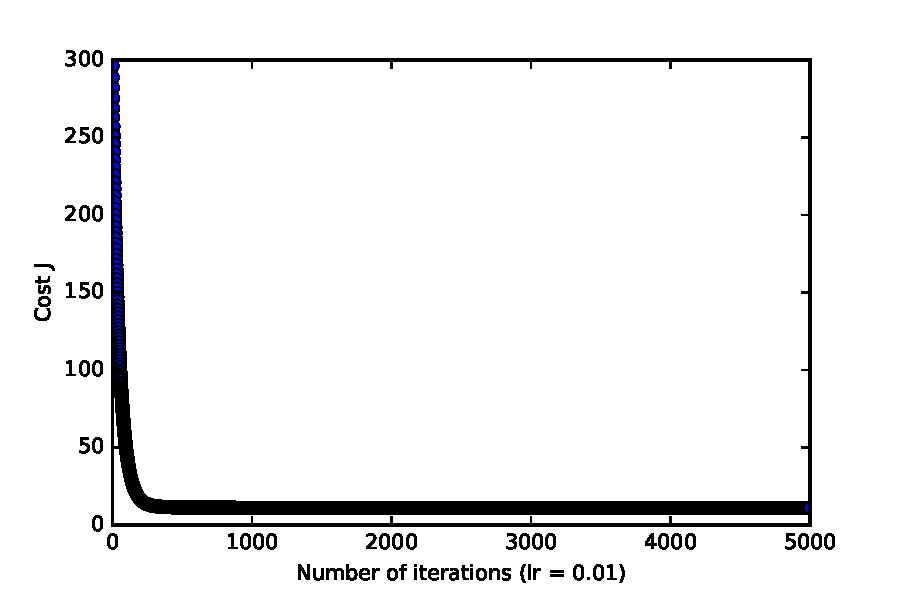
\includegraphics[scale=1]{fig001.pdf}
\end{figure}
\begin{figure}[H]
  \caption{J for different learning rate}
  \centering
    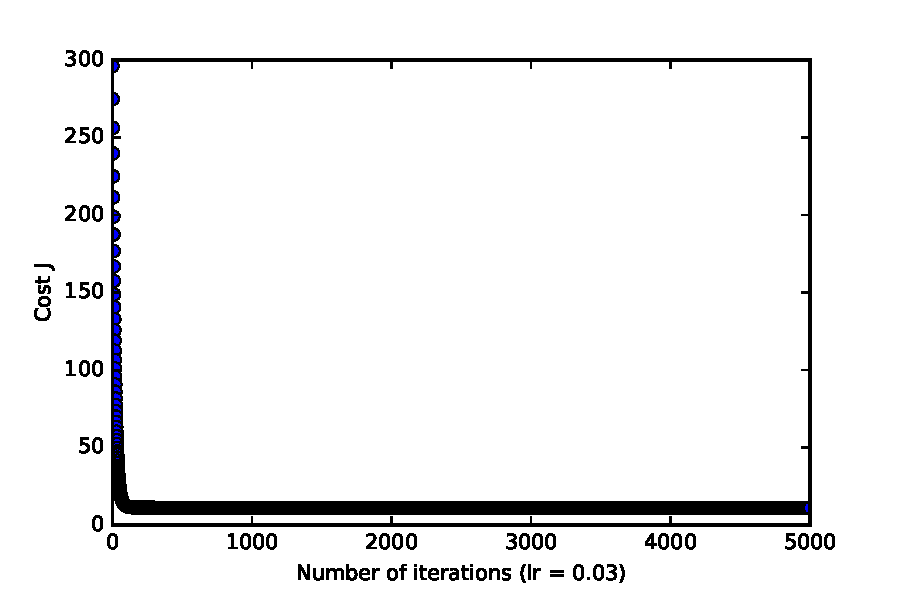
\includegraphics[scale=1]{fig003.pdf}
\end{figure}
\begin{figure}[H]
  \caption{J for different learning rate}
  \centering
    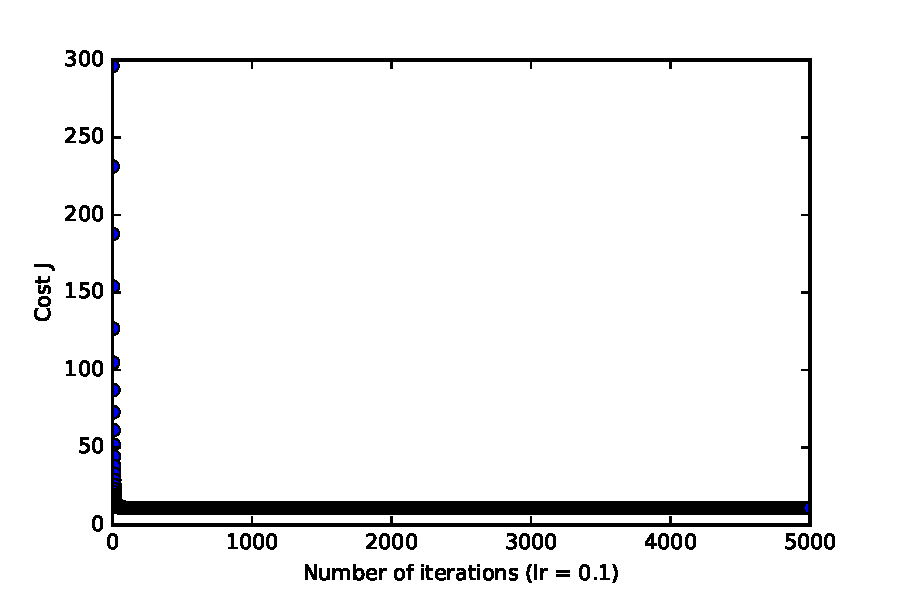
\includegraphics[scale=1]{fig01.pdf}
\end{figure}
\begin{figure}[H]
  \caption{J for different learning rate}
  \centering
    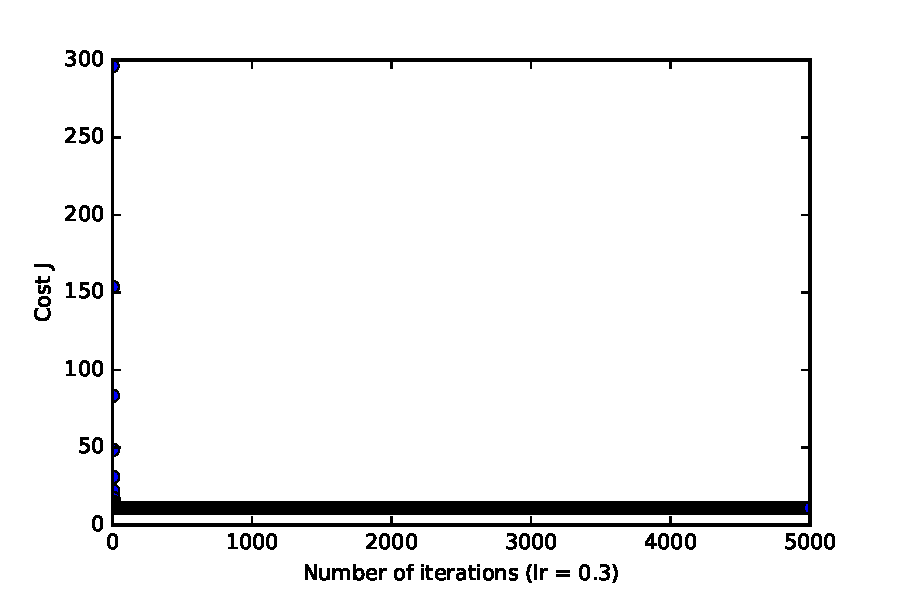
\includegraphics[scale=1]{fig03.pdf}
\end{figure}



\section{Problem 3 part 2 Implementing regularized linear regression}
\begin{figure}[H]
  \caption{JThe training data}
  \centering
    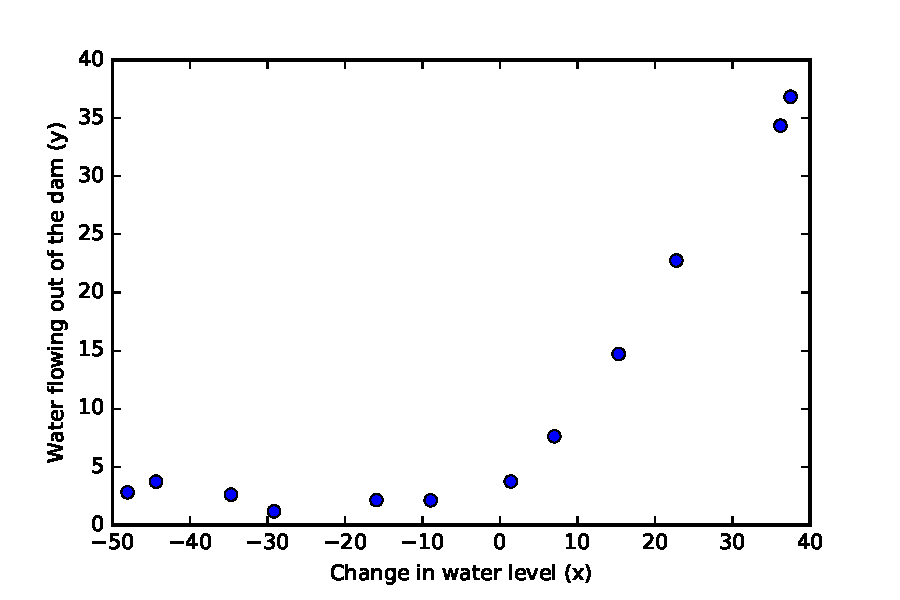
\includegraphics[scale=1]{fig6.pdf}
\end{figure}

\subsection{Problem 3.2 A1 regression cost function }
see code


\subsection{Problem 3.2 A2 Gradient of the cost function }
Learning linear regression mocel
Optimization terminated successfully.
         Current function value: 22.373906
         Iterations: 5
         Function evaluations: 6
         Gradient evaluations: 6
Theta at lambda = 0 is  [ 13.08790353   0.36777923]

\begin{figure}[H]
  \caption{The best fit for the data}
  \centering
    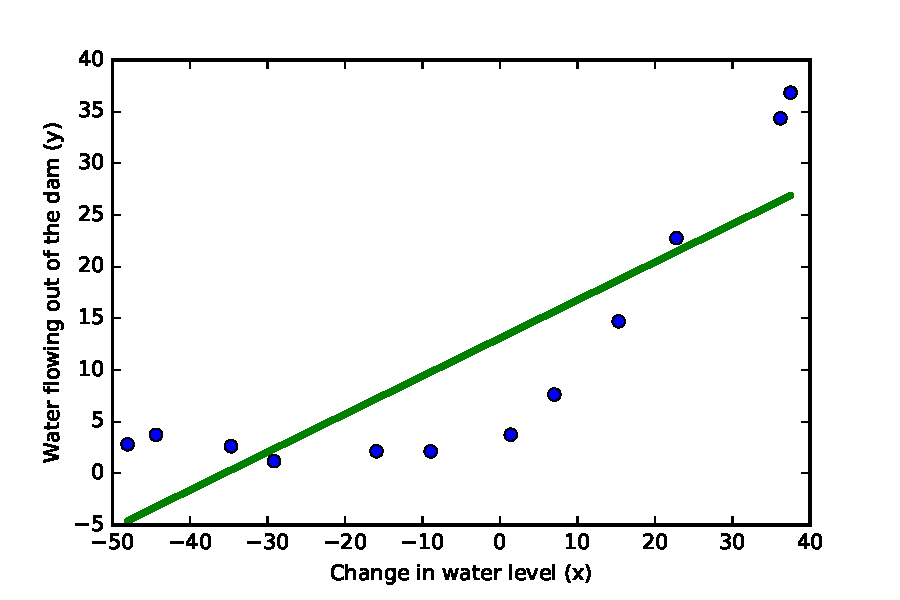
\includegraphics[scale=1]{fig7.pdf}
\end{figure}
\subsection{Problem 3.2 A3 Learning curve}

\begin{figure}[H]
  \caption{Learning curves}
  \centering
    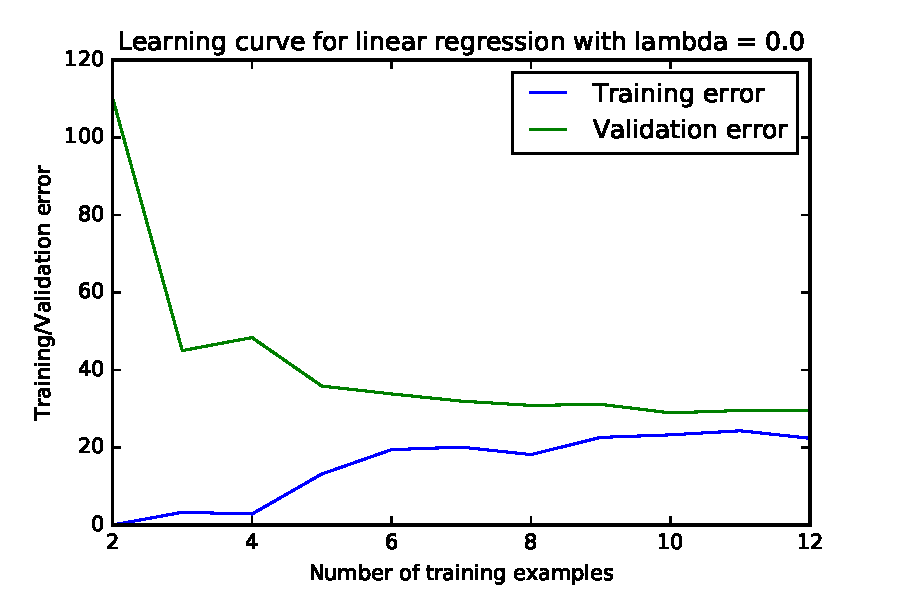
\includegraphics[scale=1]{fig8.pdf}
\end{figure}
\subsection{Learning polynomial regression models}
\begin{figure}[H]
  \caption{Polynomial fit for reg=0 with p=6}
  \centering
    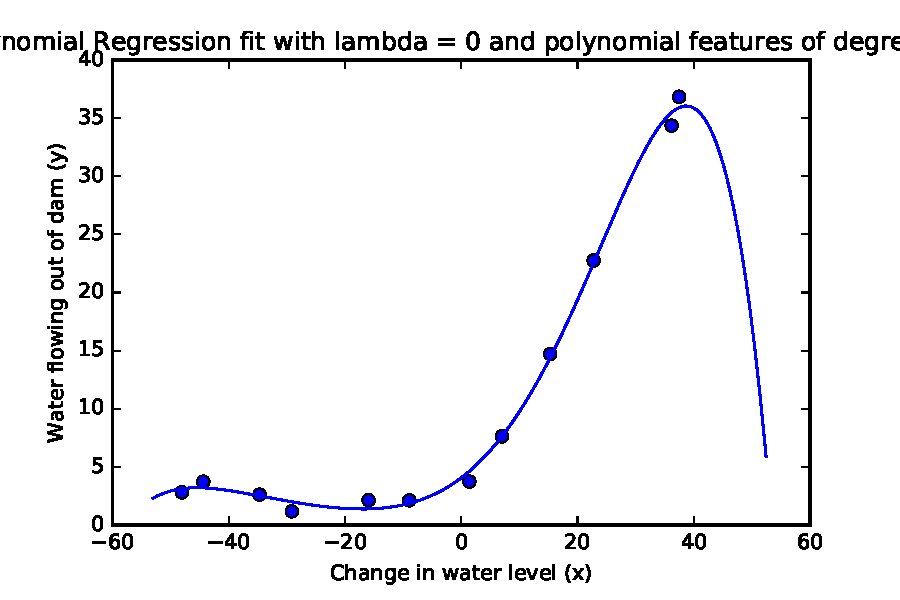
\includegraphics[scale=1]{fig9.pdf}
\end{figure}
\begin{figure}[H]
  \caption{Learning curves for reg=0}
  \centering
    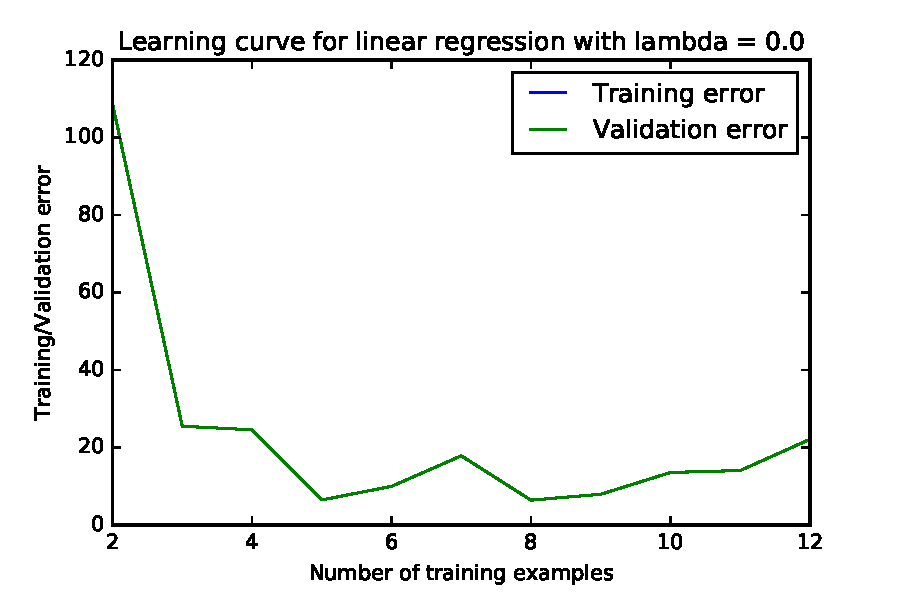
\includegraphics[scale=1]{fig10.pdf}
\end{figure}

\subsection{Problem 3.2 A4 Adjusting the regularization parameter}
We try  1,10,100
for 1:
\begin{figure}[H]
  \caption{Polynomial fit for reg=1}
  \centering
    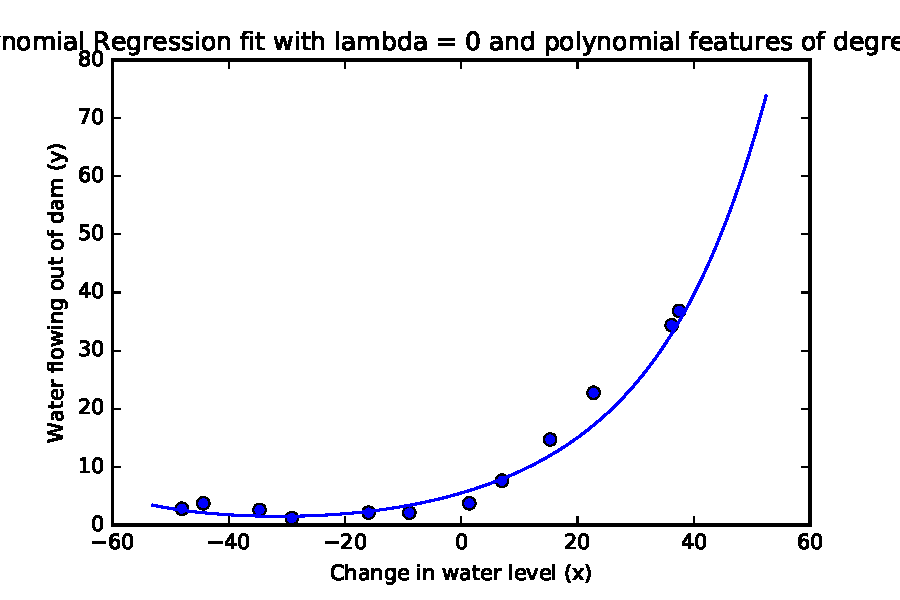
\includegraphics[scale=1]{fig91.pdf}
\end{figure}
\begin{figure}[H]
  \caption{Learning curves for reg=1}
  \centering
    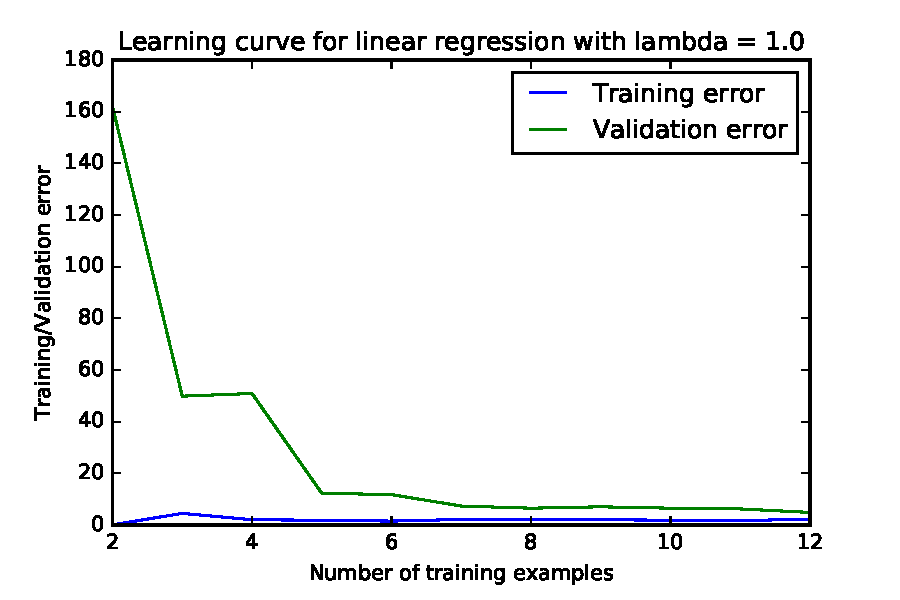
\includegraphics[scale=1]{fig101.pdf}
\end{figure}
for 10
\begin{figure}[H]
  \caption{Polynomial fit for reg=10}
  \centering
    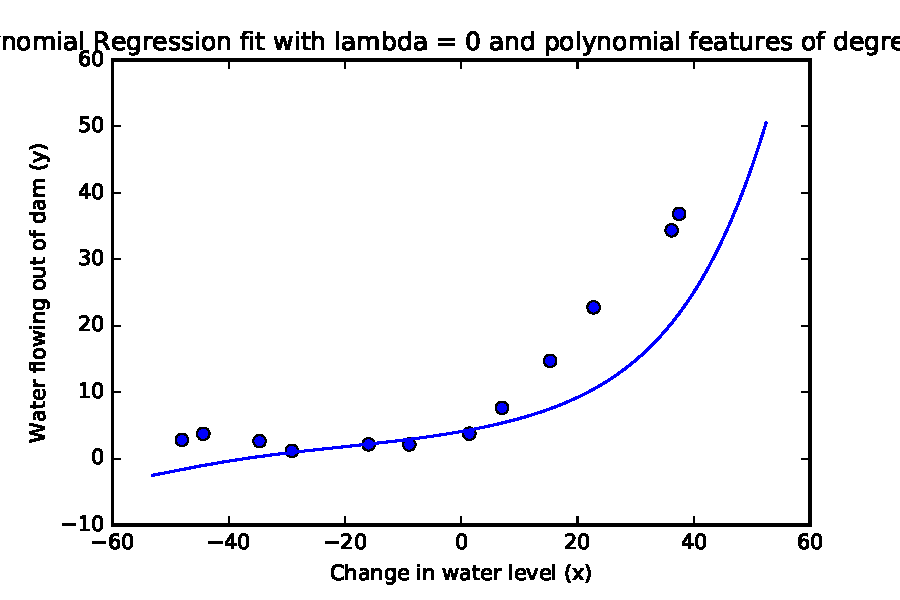
\includegraphics[scale=1]{fig910.pdf}
\end{figure}
\begin{figure}[H]
  \caption{Learning curves for reg=10}
  \centering
    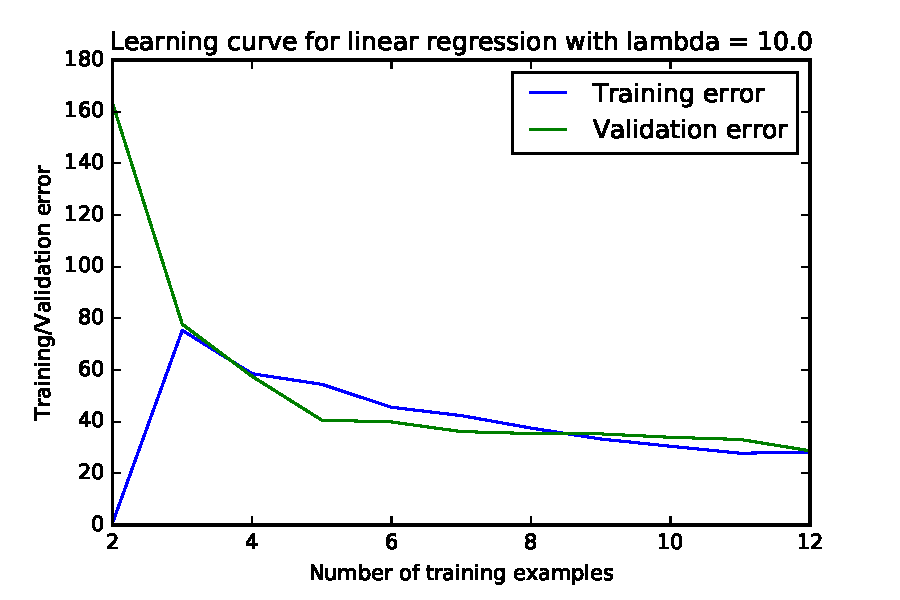
\includegraphics[scale=1]{fig1010.pdf}
\end{figure}
for 100
\begin{figure}[H]
  \caption{Polynomial fit for reg=100}
  \centering
    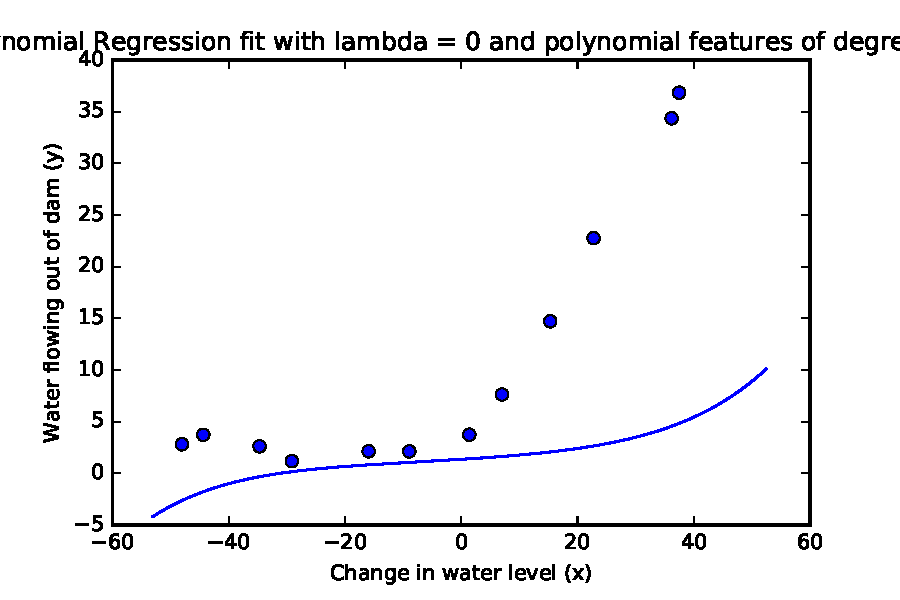
\includegraphics[scale=1]{fig9100.pdf}
\end{figure}
\begin{figure}[H]
  \caption{Learning curves for  reg=100}
  \centering
    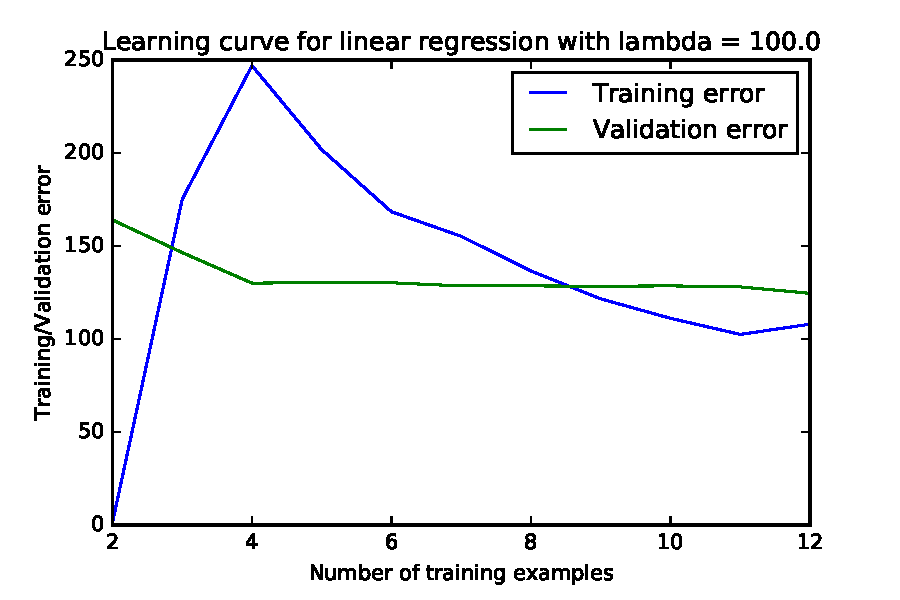
\includegraphics[scale=1]{fig10100.pdf}
\end{figure}




\subsection{Problem 3.2 A5 selecting lambda using a validation set}
Based on our error curve, We find a clear minimum for validation error between $0.3$ and $1$. As for the training data the minimum is about at $0.3$, so we make a conclusion that $0.3$ is the best choice of $\lambda$ for this problem.

\begin{figure}[H]
  \caption{Selecting lambda}
  \centering
    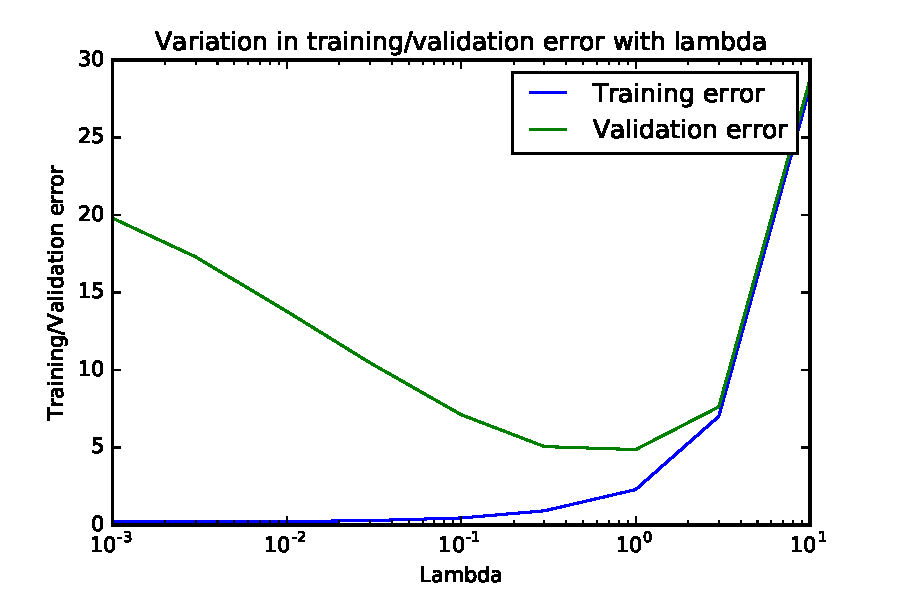
\includegraphics[scale=1]{fig12.pdf}
\end{figure}
\subsection{Problem 3.2 A6 Test error with the best model}
We find out reg=1 is the best model
\begin{figure}[H]
  \caption{Test error with the best model}
  \centering
    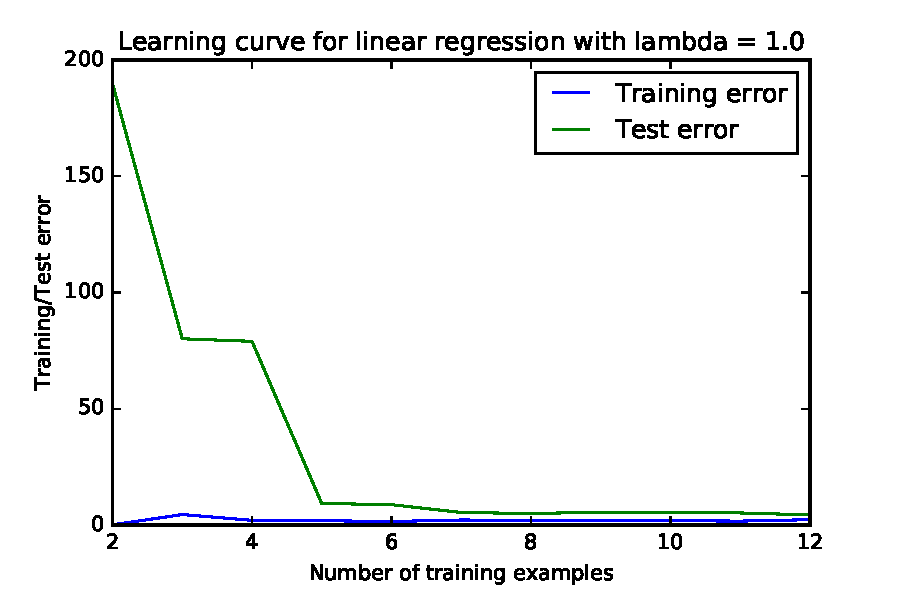
\includegraphics[scale=1]{figtest.pdf}
\end{figure}

\subsection{Problem 3.2 A6 Test error with the best model}
We plot the test error in the plot. Test error is similar to the training error
\begin{figure}[H]
  \caption{Test error with the best model}
  \centering
    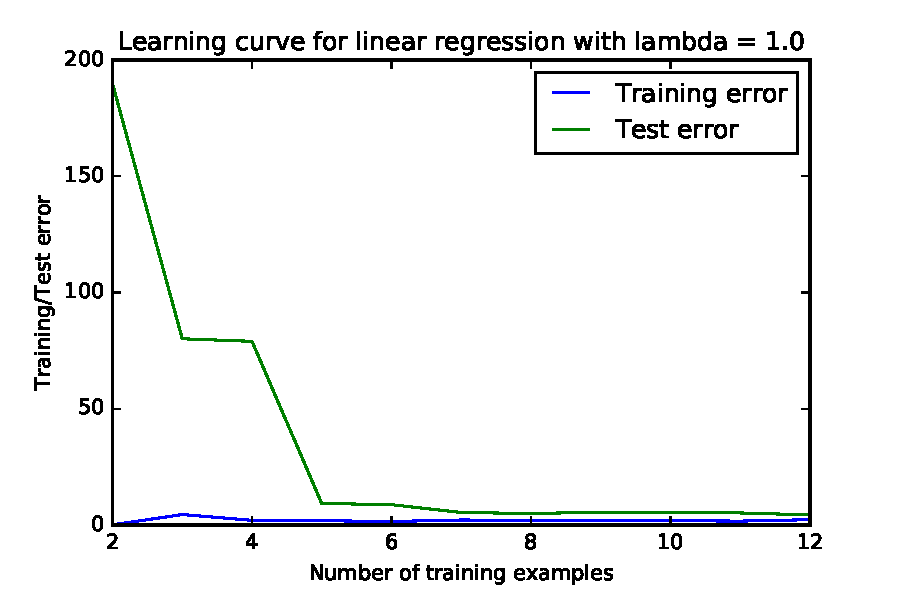
\includegraphics[scale=1]{figtest.pdf}
\end{figure}

\subsection{Problem 3.2 A7 Plotting learning curves with randomly examples}

\begin{figure}[H]
  \caption{Averaged Learning curve for lambda=1}
  \centering
    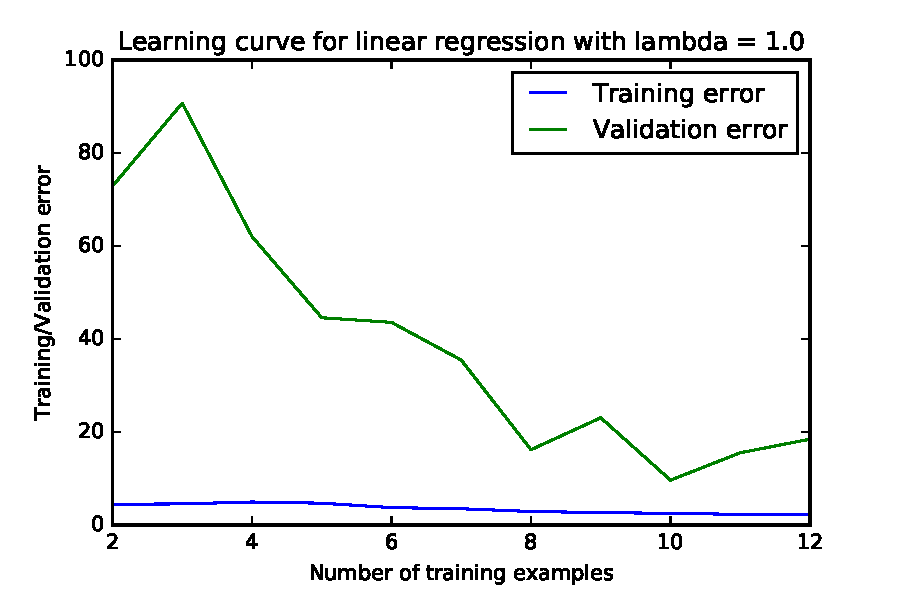
\includegraphics[scale=1]{fig11.pdf}
\end{figure}

\end{document}